\chapter[Introduction]{Introduction}
\markboth{Chap. 1\ \ \enspace Introduction}{Chap 1. Introduction}

\regularsection
\headerregularsection

\updatemylof % to be used with "list of figure divider per chapter" (see PREAMBLE)

\begin{sloppypar} % to suppress overfull box

%Lorem \index{Lorem} ipsum dolor sit amet, consectetuer adipiscing elit \cite{LIUDIMULYO201767}. Ut purus \index{purus} elit,vestibulum ut, placerat ac, adipiscing vitae, felis \citenum{LIUDIMULYO201767}. Curabitur dictum \index{dictum} gravidamauris. Nam arcu libero, nonummy eget, consectetuer id, vulputate a, magna. Donec vehicula augue eu neque \cite{liudimulyo_2018}. Pellentesque habitant morbi tristique senectuset netus et malesuada fames ac turpis egestas \index{egestas}\citenum{liudimulyo_2018}. Mauris ut leo. Cras viverra metusrhoncus sem \cite{2019liudimulyo}. Nulla et lectus vestibulum urna fringilla ultrices. Phasellus eutellus sit amet tortor gravida placerat \citenum{2019liudimulyo}. Integer sapien est, iaculis in, pretium quis,viverra ac, nunc. Praesent eget sem vel leo ultrices bibendum \cite{liudimulyo2020853}. Aenean faucibus. Morbi dolor nulla, malesuada eu, pulvinar at (\ref{fig:figures/paper-iv/fig-1}), mollis ac, nulla. Curabitur auctorsemper nulla \citenum{liudimulyo2020853}. Donec varius orci eget risus. Duis nibh mi, congue eu, accumsaneleifend, sagittis quis, diam. Duis eget orci sit amet orci dignissim rutrum \cite{LIUDIMULYO201767,liudimulyo_2018,2019liudimulyo,liudimulyo2020853,liudimulyo_unpublished1,liudimulyo_unpublished2}.


The world is progressing fast enough on technology in the last years and computer science is not 
an area that falls behind. Computer science can be divided in many areas of study, but we could 
resume  them in three big fields. Software  development,  information technology and security. 
We will be focusing on information technology such as artificial intelligence, machine learning 
and deep learning. 
\par
In  computer  science,  Artificial  Intelligence  (AI)  is  the  intelligence  carried  out  by  machines.  Its 
goal is to build smart machines capable of performing tasks that normally are made by humans.  
AI  is  just  software;  it  is  an  application  written  to  do  a  task.  For  example,  on  Facebook  with 
suggestions of names of people to tag on pictures, for fraud detection on credit cards or for self-
driving cars that can manage their shelves to drive through the city. 
\par
Artificial intelligence can be divided into two categories:
\begin{itemize}
    \item Weak AI: Sometimes referred to as “Narrow AI”, is the type of AI that only learns to do 
    one  thing,  It  is  going  to  be  better  than  a  human  doing  just  a  single  thing  such  as 
    predicting the temperature in your house to be warm but if you ask to detect a cat in a 
    picture it will be terrible.
    \item Strong  AI:  Also  known  as  General  artificial  intelligence  (AGI)  is  created  to  learn  to  do 
    anything. It is supposed to recreate the intelligence of a human, what does this mean? 
    By  this  intelligence  It  could  be  possible  to  have  a  machine  doing  the  same  things  as 
    humans like thinking or being able to take decisions. Summarizing, it is an intelligence 
    that  can  do  all  the  tasks  possible  of  doing  by  a  human.  That  is  why  it  has  not  been 
    invented yet. 
\end{itemize}


Today  there  is  weak  AI  everywhere,  Siri,  facial  recognition,  Instagram  filters,  Google  adds 
recommendations or Amazon recommendations and more examples that are taken for granted. 
Siri is a software capable of recognizing the human voice and is great at doing very few things. 
Therefore, it is not a strong AI, it is composed by a few Weak AI. This type of intelligence is better 
than a human at doing a task. For example, focusing on working out if a credit card is good or a 
fraud,  the  software  will  be more  efficient  than  a  human  just  because  it  has  processed  a wide 
dataset  of  fraudulent  or  good  cards.  Nevertheless,  the  human  will  guide  by  its  experience  or 
knowledge.
\par 
Here is where Machine learning (ML) takes part, it is the ability of a machine to learn and predict 
by  itself.  It  learns  patterns  from  the  data  to  make  the  prediction  more  accurate.  These 
algorithms can make relevant conclusions from the dataset by creating a mathematical function 
that best fits the data. The main objective of an apprentice (learner) is to develop the ability to 
generalize and associate. When we translate this into a machine or computer, it means that they 
should be able to perform accurately. One of the machine learning fields that still has a long way 
to go is deep learning. 
\par
Deep learning (DL) is a subset of machine learning that is formed of layers recreating the human 
brain. It had a breakthrough many years ago, but it came to a standstill for  some years and in 
the last few years has had a rebound. In terms of deep learning, the structure is called artificial 
neural network. DL plays with parameters, it trains a network with these parameters to learn on 
its own. By the way, after the network has been trained it will be able to recognize patterns in 
the  input  data  to  make  the  detection  accurate.
\par
In deep learning there is a very large and important study area that has gained a lot of strength 
in  recent  years,  object  detection  in  real  time.  It  is  mainly  used  in  video  vigilance  cameras  of 
highways  or  for  autonomous  cars  cameras.  It  consists  in  the  capacity  of  a  machine  to  detect 
objects in a set of images in a very small processing time. The  network’s  capacity  of 
generalization must be very good because skipping the detection of an object in an image is a 
sign  of  loss  of  accuracy.  This  final  degree  project  will  be  focusing  on  detecting  vehicles  (cars, 
trucks, motorcycles) in videos and then tracking those vehicles to be able to count them. Video 
processing must be done in record time to be in real-time. 

\end{sloppypar}

%\begin{figure} % \begin{figure} will let LaTeX decide the best figure placement for you ; \begin{figure}[H] for forcing the figure placement here ; in the bottom, \begin{figure}[!b] ; top of the page, \begin{figure}[!t]
%    \centering
%    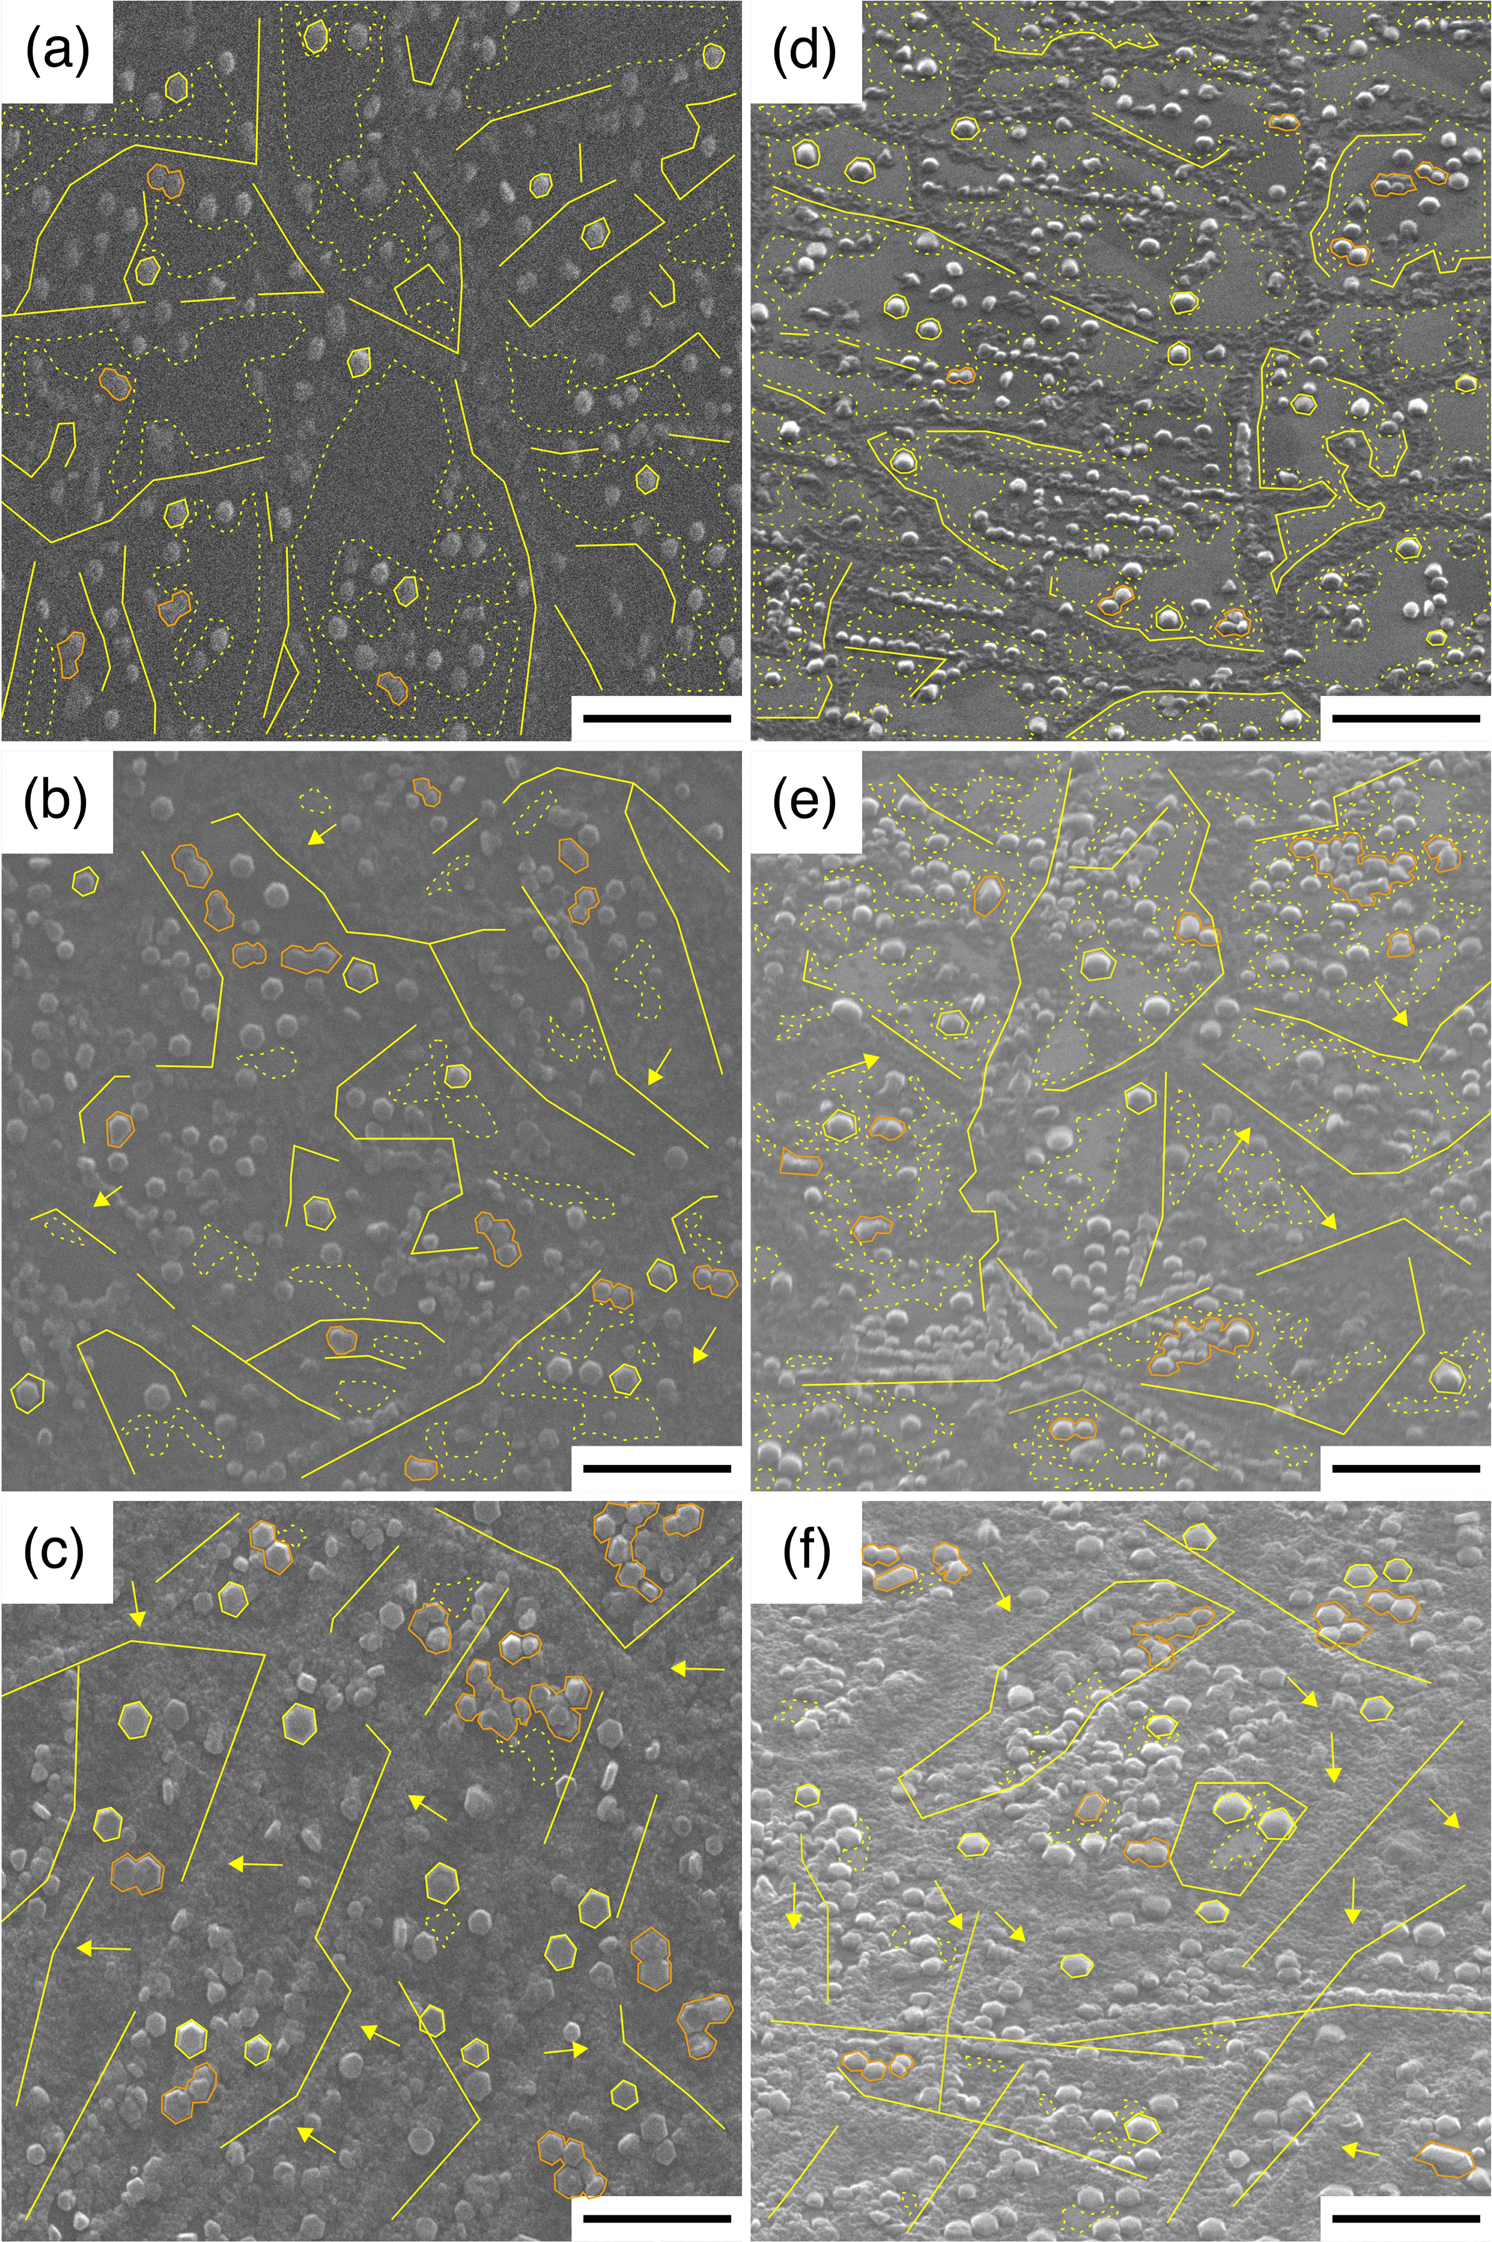
\includegraphics[width=0.95\textwidth]{figures/paper-iv/fig-1.png}
%    \caption[SEM images of AlN on graphene formed via different MEE cycles]{SEM images of AlN on graphene formed via different MEE cycles. (\textbf{a},\textbf{d}), (\textbf{b},\textbf{e}) and (\textbf{c},\textbf{f}) are (top-, bird’s eye-view) SEM images of samples A1, A2 and A3, respectively. Scale bars are 1 {\textmu}m. Features marked with yellow lines, yellow (orange) contours and yellow dashed outlines are high-density AlN nanostructures grown along line defects of graphene, individual (coalesced) AlN islands and areas of exposed graphene, respectively. Yellow arrows in samples A2 and A3 show the lateral growth of AlN nanostructures that initially nucleate at the line defects of graphene in sample A1 (adapted with permission from ref. \citenum{liudimulyo2020853} \copyright \ Liudi Mulyo \textit{et al}, 2020.}
%    \label{fig:figures/paper-iv/fig-1}
%\end{figure}

%\section{Section 1 in chapter 1}
%\lipsum[2]

%\begin{equation}
%    EQE = \frac{q \times P_{opt}}{I \times h\nu}
%\end{equation}

%\lipsum[3-4]

%\subsection{Subsection 1.1 of section 1 in chapter 1}
%\lipsum[5-7]

%\subsection{Subsection 1.2 of section 1 in chapter 1}
%\lipsum[8-10]

%\clearpage\phantomsection % to fix wrong hyperref to this section
%\section[Long section title displayed in the table of content]{Short section title in the chapter}
%\sectionmark{Even shorter title on the header}
%\lipsum[11-20]

%\subsection{Subsection 1.2 of section 2 in chapter 1}
%\lipsum[13-14]

%=======================================================================
%%% References 

% \clearpage
\phantomsection
\specialsection % put an indent, see preamble
\headerspecialsection

{\hypersetup{urlcolor=ntnu,linkcolor=sophia} % set clickable URL title color to black, not ntnu like in the main document

\bibliographystyle{unsrtnat-mod}  % NATBIB ref style
\bibliography{references}
}
